% -------------------------------------------------------
\section{Эксперимент 2: Задача выбора карточек Уэйсона}
% -------------------------------------------------------

\subsection{Обоснование выбора парадигмы}

Задача выбора карточек Уэйсона~\cite{wason1966reasoning} была выбрана как каноническая парадигма для исследования предубеждения подтверждения в дедуктивном рассуждении. В оригинальной версии испытуемым предъявляются четыре карточки, соответствующие случаям P, $\lnot$P, Q и $\lnot$Q, и условное правило «если P, то Q». Нормативно правильный ответ --- выбор карточек P и $\lnot$Q --- позволяет фальсифицировать правило.

Эмпирическое распределение ответов людей в абстрактной версии задачи хорошо задокументировано. Мета-анализ Ragni и соавторов, обобщивший 228 экспериментов~\cite{ragni2018experimental}, показал, что лишь $\approx$19\% участников решают абстрактную задачу правильно; в оригинальной выборке Wason и Shapiro (1971) этот показатель составляет $\approx$4\%~\cite{wason1971natural}. Доминирующим паттерном ошибки является matching bias~\cite{evans1998matching} --- выбор карточек P и Q, буквально упомянутых в правиле. Таблица~\ref{tab:human_wason} обобщает распределение ответов людей по основным категориям.

\begin{table}[h!]
\caption{Распределение ответов людей в задаче выбора Уэйсона (абстрактная версия). Данные: мета-анализ Ragni et al. (2018)~\cite{ragni2018experimental}, 228 экспериментов; оригинальная выборка Wason \& Shapiro (1971)~\cite{wason1971natural}; Evans (1998)~\cite{evans1998matching}}
\label{tab:human_wason}
\centering
\begin{tabular}{|l|c|c|l|}
\hline
\textbf{Паттерн выбора} & \textbf{Мета-анализ} & \textbf{Оригинал} & \textbf{Интерпретация} \\
\hline
P + $\lnot$Q (правильный) & 19\% & $\approx$4\% & Нормативный ответ \\
P + Q (matching bias) & 39\% & $\approx$45\% & Выбор упомянутых в правиле \\
P только (confirmation) & 36\% & $\approx$35\% & Минимальное подтверждение \\
P + Q + $\lnot$Q & 5\% & $\approx$7\% & Частичный matching \\
Прочие комбинации & 1\% & $\approx$3\% & Неклассифицируемые \\
\hline
\end{tabular}
\end{table}

Критически важным для интерпретации результатов LLM является контент-эффект: при деонтическом framing (социальные контракты) доля правильных ответов у людей возрастает до $\approx$64\%~\cite{ragni2018experimental}, а matching bias снижается. Данный паттерн воспроизводится и в настоящем эксперименте, что позволяет говорить о качественном сходстве механизмов фасилитации.

Задача обеспечивает прямую операционализацию предубеждения подтверждения~\cite{nickerson1998confirmation}: выбор карточек P и Q отражает поиск подтверждающих, а не фальсифицирующих свидетельств. Кроме того, задача позволяет исследовать контент-эффекты~\cite{cheng1985pragmatic, cosmides1992cognitive}: известно, что задачи с содержанием социальных контрактов решаются людьми значительно лучше, чем абстрактные версии.

\subsection{Конструкция стимульных датасетов: четыре контентных условия}

Были сконструированы пять стимульных датасетов, каждый включающий 100--101 уникальное условное правило с соответствующими отображениями на четыре позиции карточек.

\textbf{Формальная логика --- Каноническая.} Правила используют стандартные абстрактные символы из классической литературы по задаче Уэйсона (буквы, числа, геометрические фигуры). Условие включено для сравнения с предшествующими работами при признании риска контаминации~\cite{arkoudas2023gpt4}.

\textbf{Формальная логика --- Нейтральная.} Правила используют оригинальные абстрактные пары, не присутствующие в канонических формулировках (например, «если символ является Стрелкой, то узор является Полосатым»). Это условие служит деконтаминированным абстрактным базисом и непосредственно адресует методологический пробел работ, опирающихся исключительно на канонические стимулы.

\textbf{Конкретные факты.} Правила основаны на верифицируемых реальных свойствах объектов (например, «если животное является дельфином, то оно дышит воздухом»). Условие операционализирует семантические априорные знания без введения нормативных социальных обязательств.

\textbf{Знакомые социальные контракты.} Деонтические правила, отражающие широко известные социальные нормы и институциональные разрешения (например, «если человек управляет автомобилем, то у него должны быть права»). Условие воспроизводит эффект фасилитации, описанный Ченгом и Холиоаком~\cite{cheng1985pragmatic}. Из набора исключены юрисдикционно-специфические правила.

\textbf{Незнакомые фантастические социальные контракты.} Деонтические правила, вписанные в вымышленные миры, не пересекающиеся с известными художественными вселенными (например, «если путешественник пересекает Лунные ворота, он должен нести Серебряное перо»). Условие разработано для диссоциации двух конкурирующих объяснений эффекта социального контракта: знакомость конкретного содержания правила или распознавание деонтической структуры разрешения/обязательства~\cite{cheng1985pragmatic, cosmides1992cognitive}. Насколько известно автору, подобное условие ранее не реализовывалось в исследованиях LLM.

Ключевым методологическим вкладом дизайна является систематическая манипуляция порядком предъявления карточек. Каждый стимул предъявлялся каждой модели в \textbf{пяти различных перестановках} четырёх позиций карточек. Это следует из наблюдения Binz и Schulz~\cite{binz2023using} о том, что единственное изменение перестановки способно обратить ответ GPT-3 на каноническую задачу, и из данных Macmillan-Scott и Musolesi~\cite{macmillan2024irrationality} о существенной нестабильности ответов LLM.

Данный дизайн даёт \textbf{500 испытаний на модель на условие} (100 правил $\times$ 5 перестановок), позволяя оценивать распределения ответов, а не точечные оценки, и разделять правильность и стабильность как независимые свойства поведения модели.

\subsection{Промпт-условия}

Оценивались три промпт-условия на датасете «Формальная логика --- Нейтральная».

\textbf{Original (Assisted Falsification).} Системный промпт задаёт персону эксперта по логике и явную задачу найти карточки, нарушающие правило:

\begin{quote}
\textit{System: You are a logic expert analyzing conditional rules. Your task is to identify which cards must be turned over to check if a rule is violated. CRITICAL INSTRUCTIONS: Respond ONLY with the selected cards as a comma-separated list. NO explanations, NO reasoning, NO JSON, NO other text.}
\end{quote}

Условие обеспечивает два независимых фасилитирующих сигнала: ролевое прайминирование и явный фрейминг фальсификации. Служит верхней границей производительности без CoT и позволяет сравниться с предшествующими работами, большинство из которых используют аналогично директивные промпты.

\textbf{Neutral.} Системный промпт содержит только инструкцию по формату без персоны и без фрейминга фальсификации:

\begin{quote}
\textit{System: Respond ONLY with card labels as a comma-separated list. No explanations.}
\end{quote}

Наиболее близко воспроизводит оригинальную человеческую экспериментальную парадигму и служит основным измерением непромпт-ированной логической компетентности.

\textbf{Chain-of-Thought (CoT).} Системный промпт инструктирует модель рассуждать пошагово и выводить финальный ответ в фиксированном формате~\cite{wei2022chain}:

\begin{quote}
\textit{System: You are a logic expert analyzing conditional rules. Think step by step before answering. After reasoning, output your final answer on the last line as: ANSWER: card1, card2.}
\end{quote}

Условие CoT тестирует, раскрывает ли явное элицирование рассуждений латентную компетентность у моделей, недостаточно показывающих себя при прямых ответах, и взаимодействует ли CoT дифференцированно с уровнем способностей модели~\cite{kojima2022large}.

Все модели запрашивались с temperature~=~1{,}0 для сохранения естественной вариабельности ответов между перестановками. Примеры не предоставлялись; все условия --- zero-shot.

\subsection{Метрики}

\textbf{Expected Metric Accuracy (EMA)} --- доля испытаний, в которых модель выбирает ровно нормативно правильный набор карточек $\{$P, $\lnot$Q$\}$. Основная мера логической правильности, сопоставимая с метриками точности в работах Dasgupta и соавторов~\cite{dasgupta2024language} и Macmillan-Scott и Musolesi~\cite{macmillan2024irrationality}.

\textbf{Matching Bias Index (MBI)} --- доля испытаний, в которых модель выбирает $\{$P, Q$\}$ --- карточки, явно упомянутые в правиле~\cite{evans1998matching}. Операционализирует предубеждение соответствия.

\textbf{Confirmation Bias Rate (CBR)} --- доля испытаний, в которых модель выбирает только $\{$P$\}$ --- минимальный подтверждающий выбор. Совместно с MBI формирует «семейство предубеждения подтверждения».

\textbf{Consistency Rate} --- доля правил, для которых модель даёт идентичный выбор карточек во всех пяти перестановках. Количественно оценивает стабильность ответов независимо от правильности.

\subsection{Результаты и анализ}

\textbf{Результаты по контентным условиям.} Полные данные по всем пяти датасетам приведены в таблице~\ref{tab:wst_content1} и на рисунке~\ref{fig:ema_conditions}.

\begin{figure}[h!]
\centering
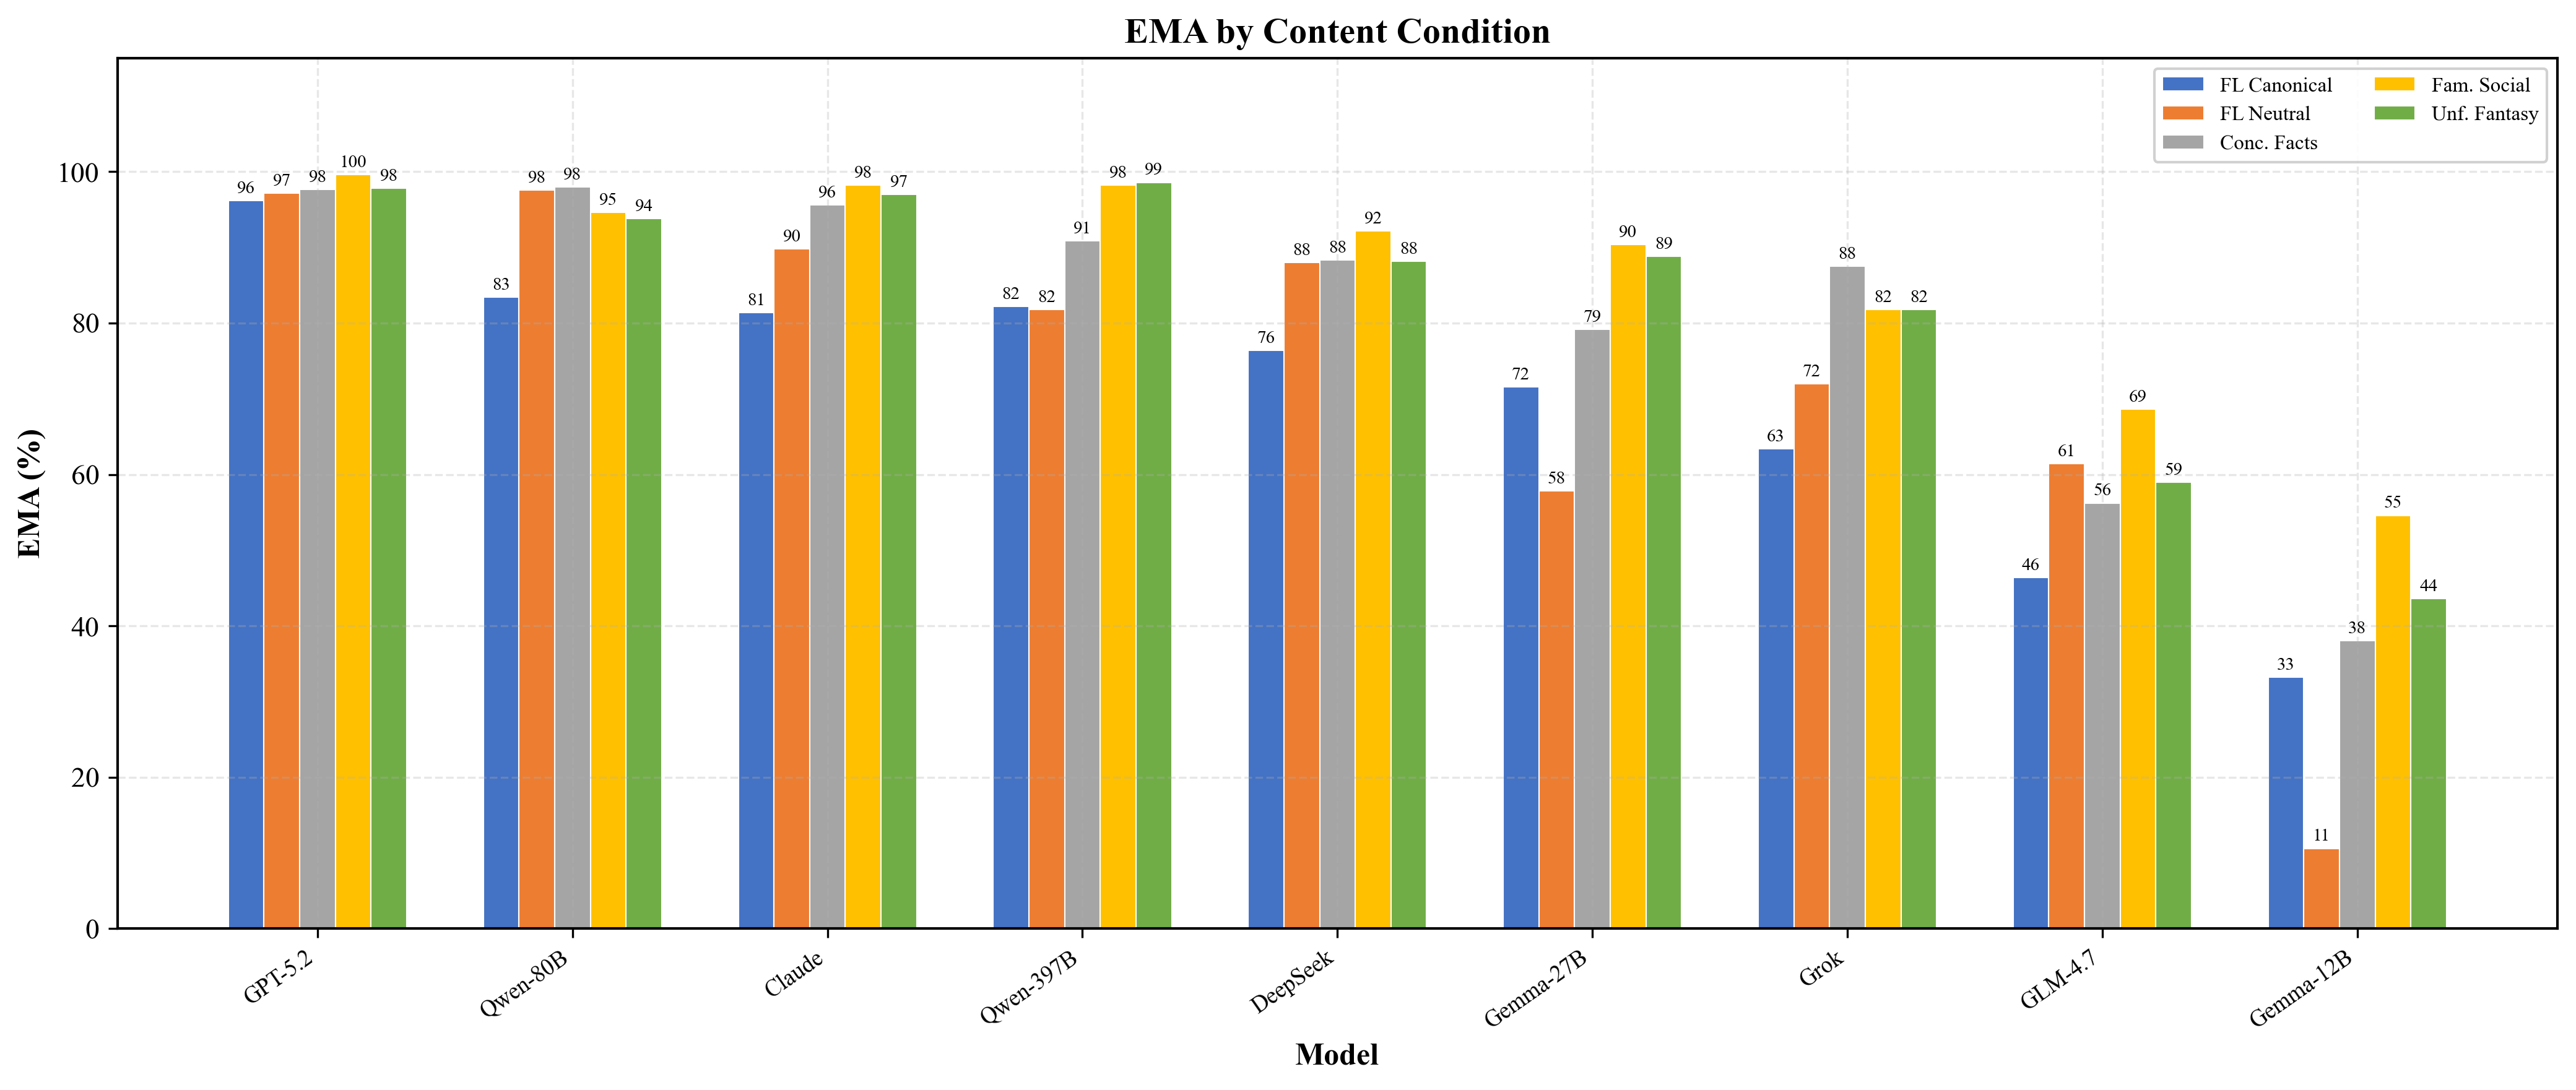
\includegraphics[width=0.95\textwidth]{../experiments_raw_results/wason-selection/figures/wason_ema_conditions.png}
\caption{EMA по пяти контентным условиям для всех девяти моделей. Модели отсортированы по убыванию EMA в FL Neutral. Значения выше 0{,}90 достигаются топовыми моделями во всех условиях, в то время как слабые модели демонстрируют значительный разброс в зависимости от контента.}
\label{fig:ema_conditions}
\end{figure}

\begin{figure}[h!]
\centering
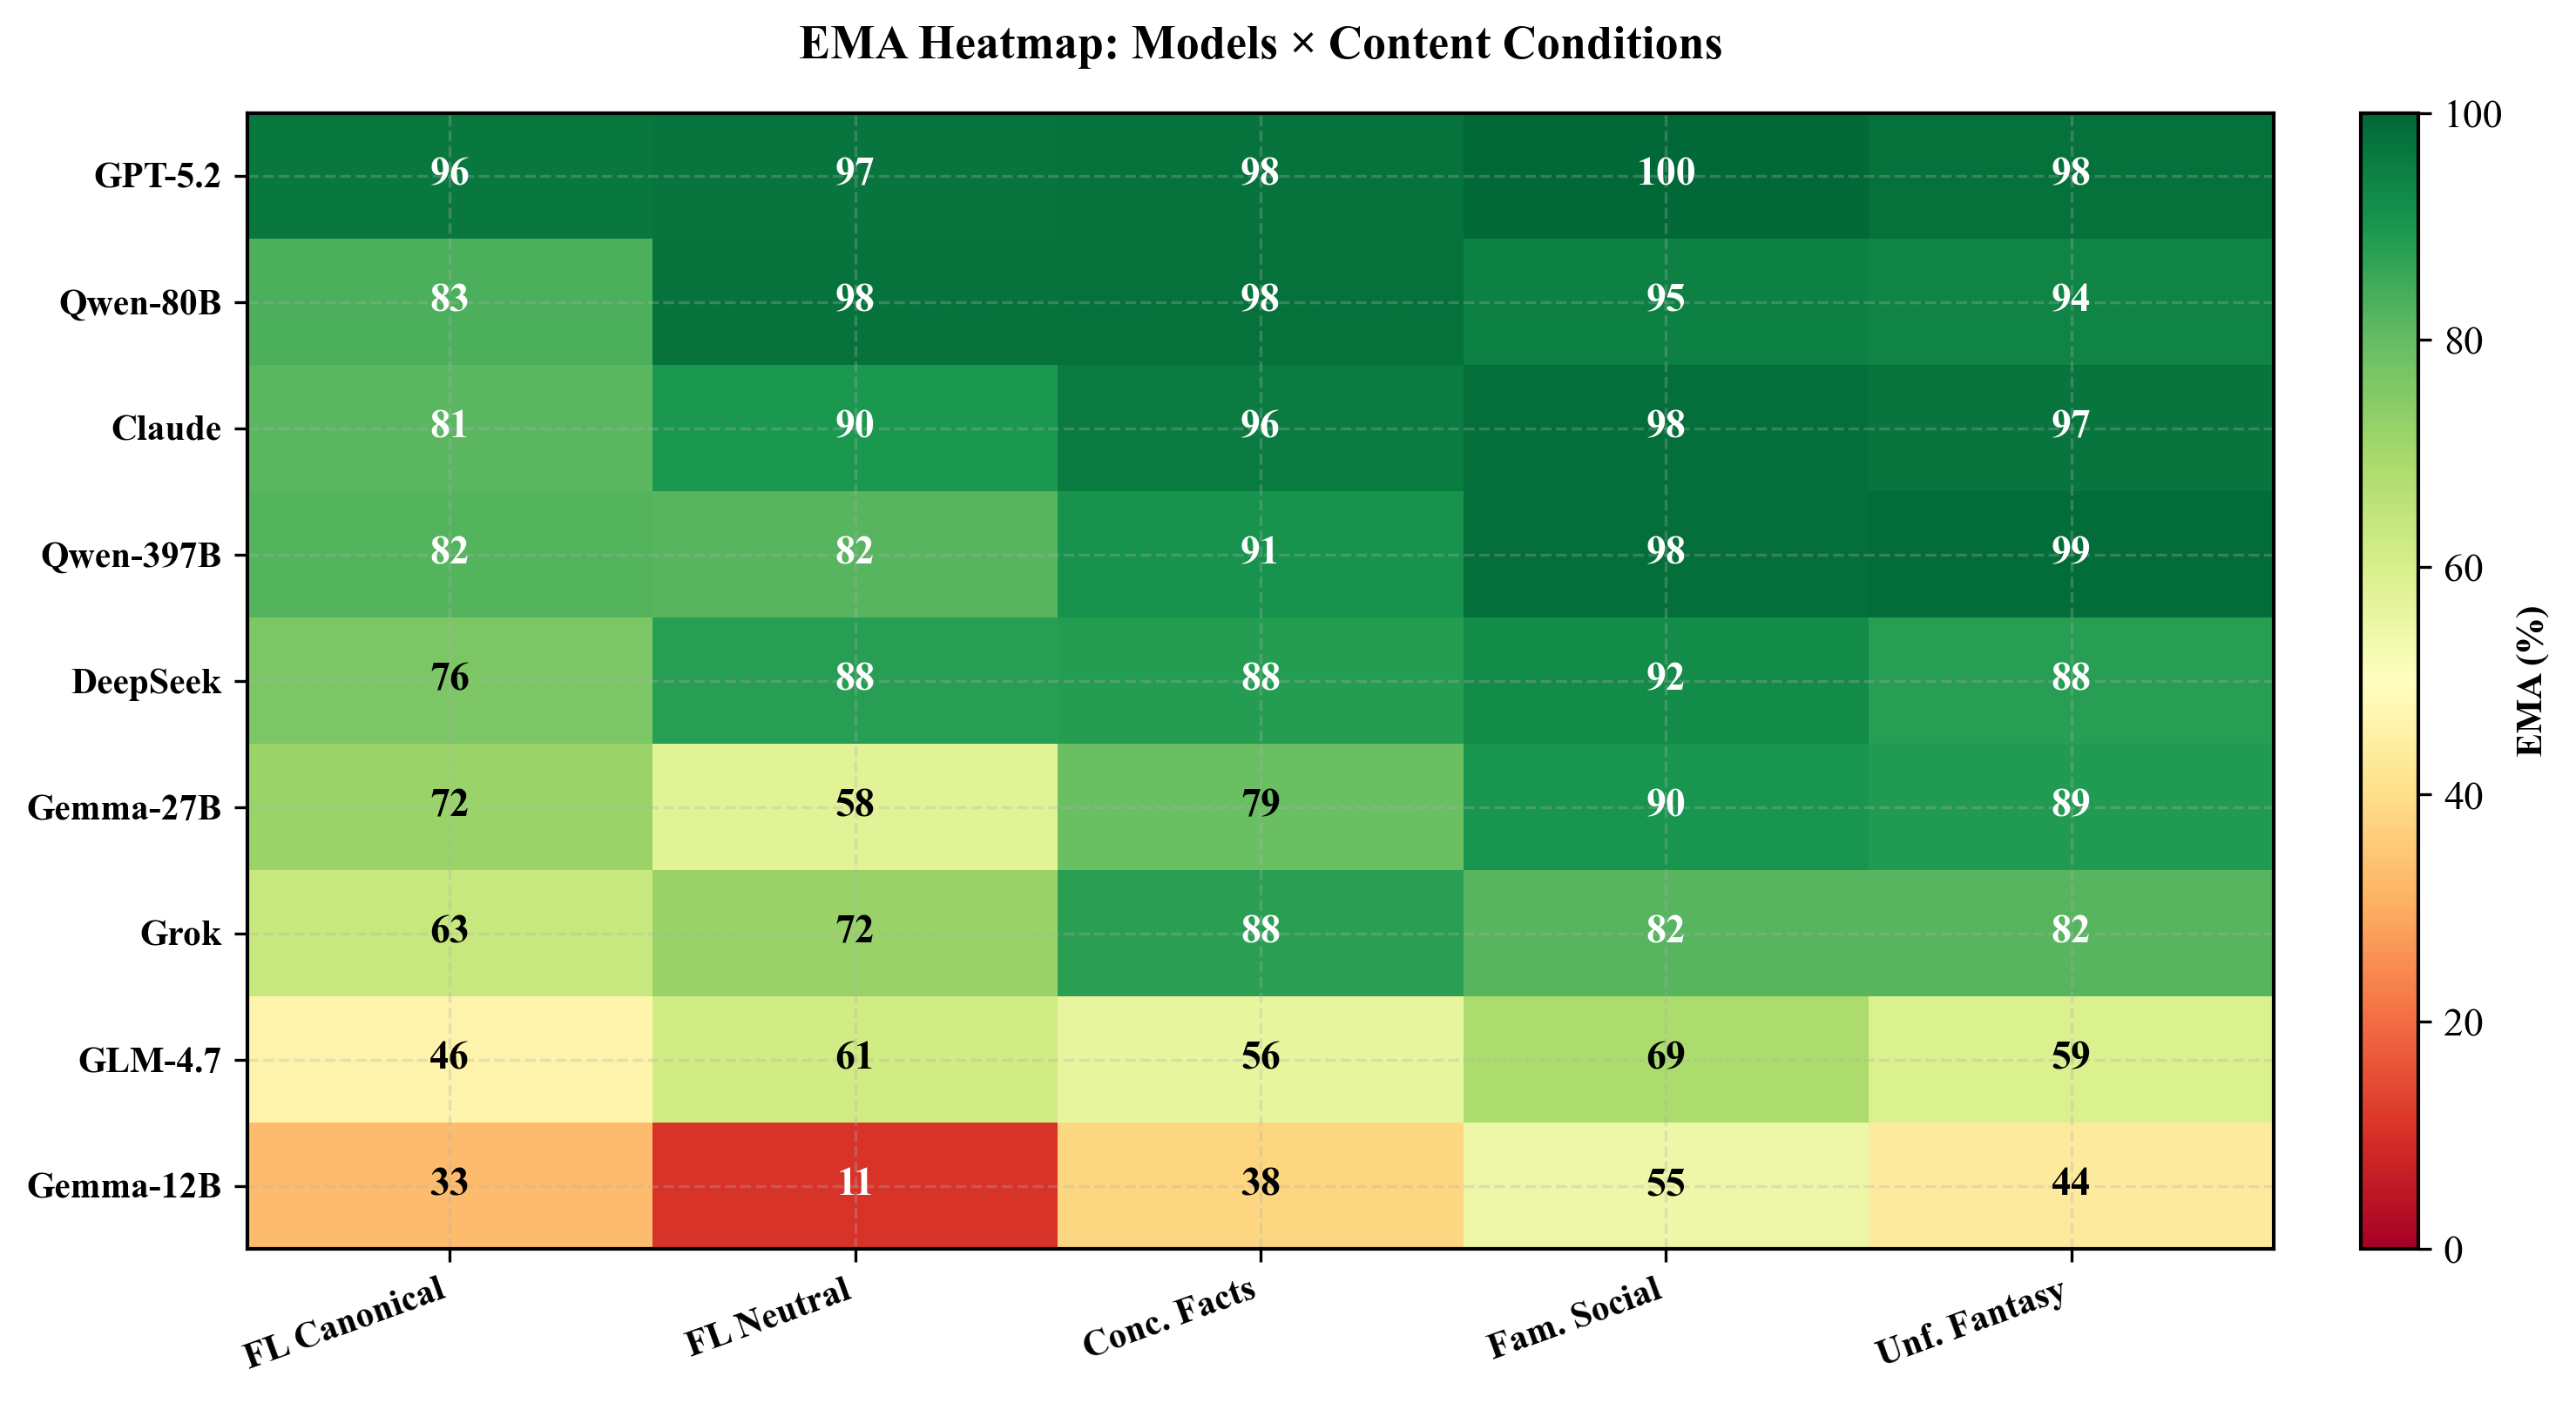
\includegraphics[width=0.95\textwidth]{../experiments_raw_results/wason-selection/figures/wason_ema_heatmap.png}
\caption{Тепловая карта EMA: модели $\times$ контентные условия. Визуализация подчёркивает универсальность контент-эффекта --- все модели без исключения показывают более светлые ячейки в условиях с семантическим содержанием по сравнению с абстрактными.}
\label{fig:ema_heatmap}
\end{figure}

\begin{table}[h!]
\caption{EMA по пяти контентным условиям}
\label{tab:wst_content1}
\centering
\begin{tabular}{|l|c|c|c|c|c|}
\hline
\textbf{Модель} & \textbf{FL Canon.} & \textbf{FL Neutral} & \textbf{Conc. Facts} & \textbf{Fam. Social} & \textbf{Unf. Fantasy} \\
\hline
gpt-5.2                   & 0,973 & 0,972 & 0,976 & 0,996 & 0,978 \\
qwen3-next-80b            & 0,933 & 0,976 & 0,980 & 0,946 & 0,938 \\
qwen3.5-397b-a17b         & 0,867 & 0,818 & 0,909 & 0,982 & 0,986 \\
claude-sonnet-4.6         & 0,907 & 0,898 & 0,956 & 0,982 & 0,970 \\
deepseek-v3.2             & 0,847 & 0,880 & 0,883 & 0,922 & 0,882 \\
grok-4.1-fast             & 0,647 & 0,720 & 0,875 & 0,818 & 0,818 \\
gemma-3-27b-it            & 0,553 & 0,578 & 0,792 & 0,904 & 0,888 \\
glm-4.7-flash             & 0,533 & 0,614 & 0,562 & 0,686 & 0,590 \\
gemma-3-12b-it            & 0,207 & 0,106 & 0,380 & 0,546 & 0,436 \\
\hline
\end{tabular}
\end{table}

\textbf{Контент-эффект} является наиболее устойчивым результатом эксперимента и воспроизводится у всех девяти моделей. Переход от абстрактного нейтрального условия к знакомым социальным контрактам даёт прирост EMA у восьми из девяти моделей (медианный прирост $+0{,}084$): от снижения на $-0{,}030$ у \texttt{qwen3-next-80b} (у которой EMA и так близка к потолку $0{,}976$) до $+0{,}440$ у \texttt{gemma-3-12b-it}. Критически важным является результат условия «Незнакомых фантастических социальных контрактов»: EMA в нём превышает EMA в нейтральном абстрактном условии у семи из девяти моделей (медианный прирост $+0{,}072$) и вплотную приближается к EMA знакомых социальных контрактов. Это поддерживает гипотезу прагматических схем~\cite{cheng1985pragmatic}: деонтическая структура обязательства фасилитирует правильный логический вывод независимо от знакомости содержания.

\begin{figure}[h!]
\centering
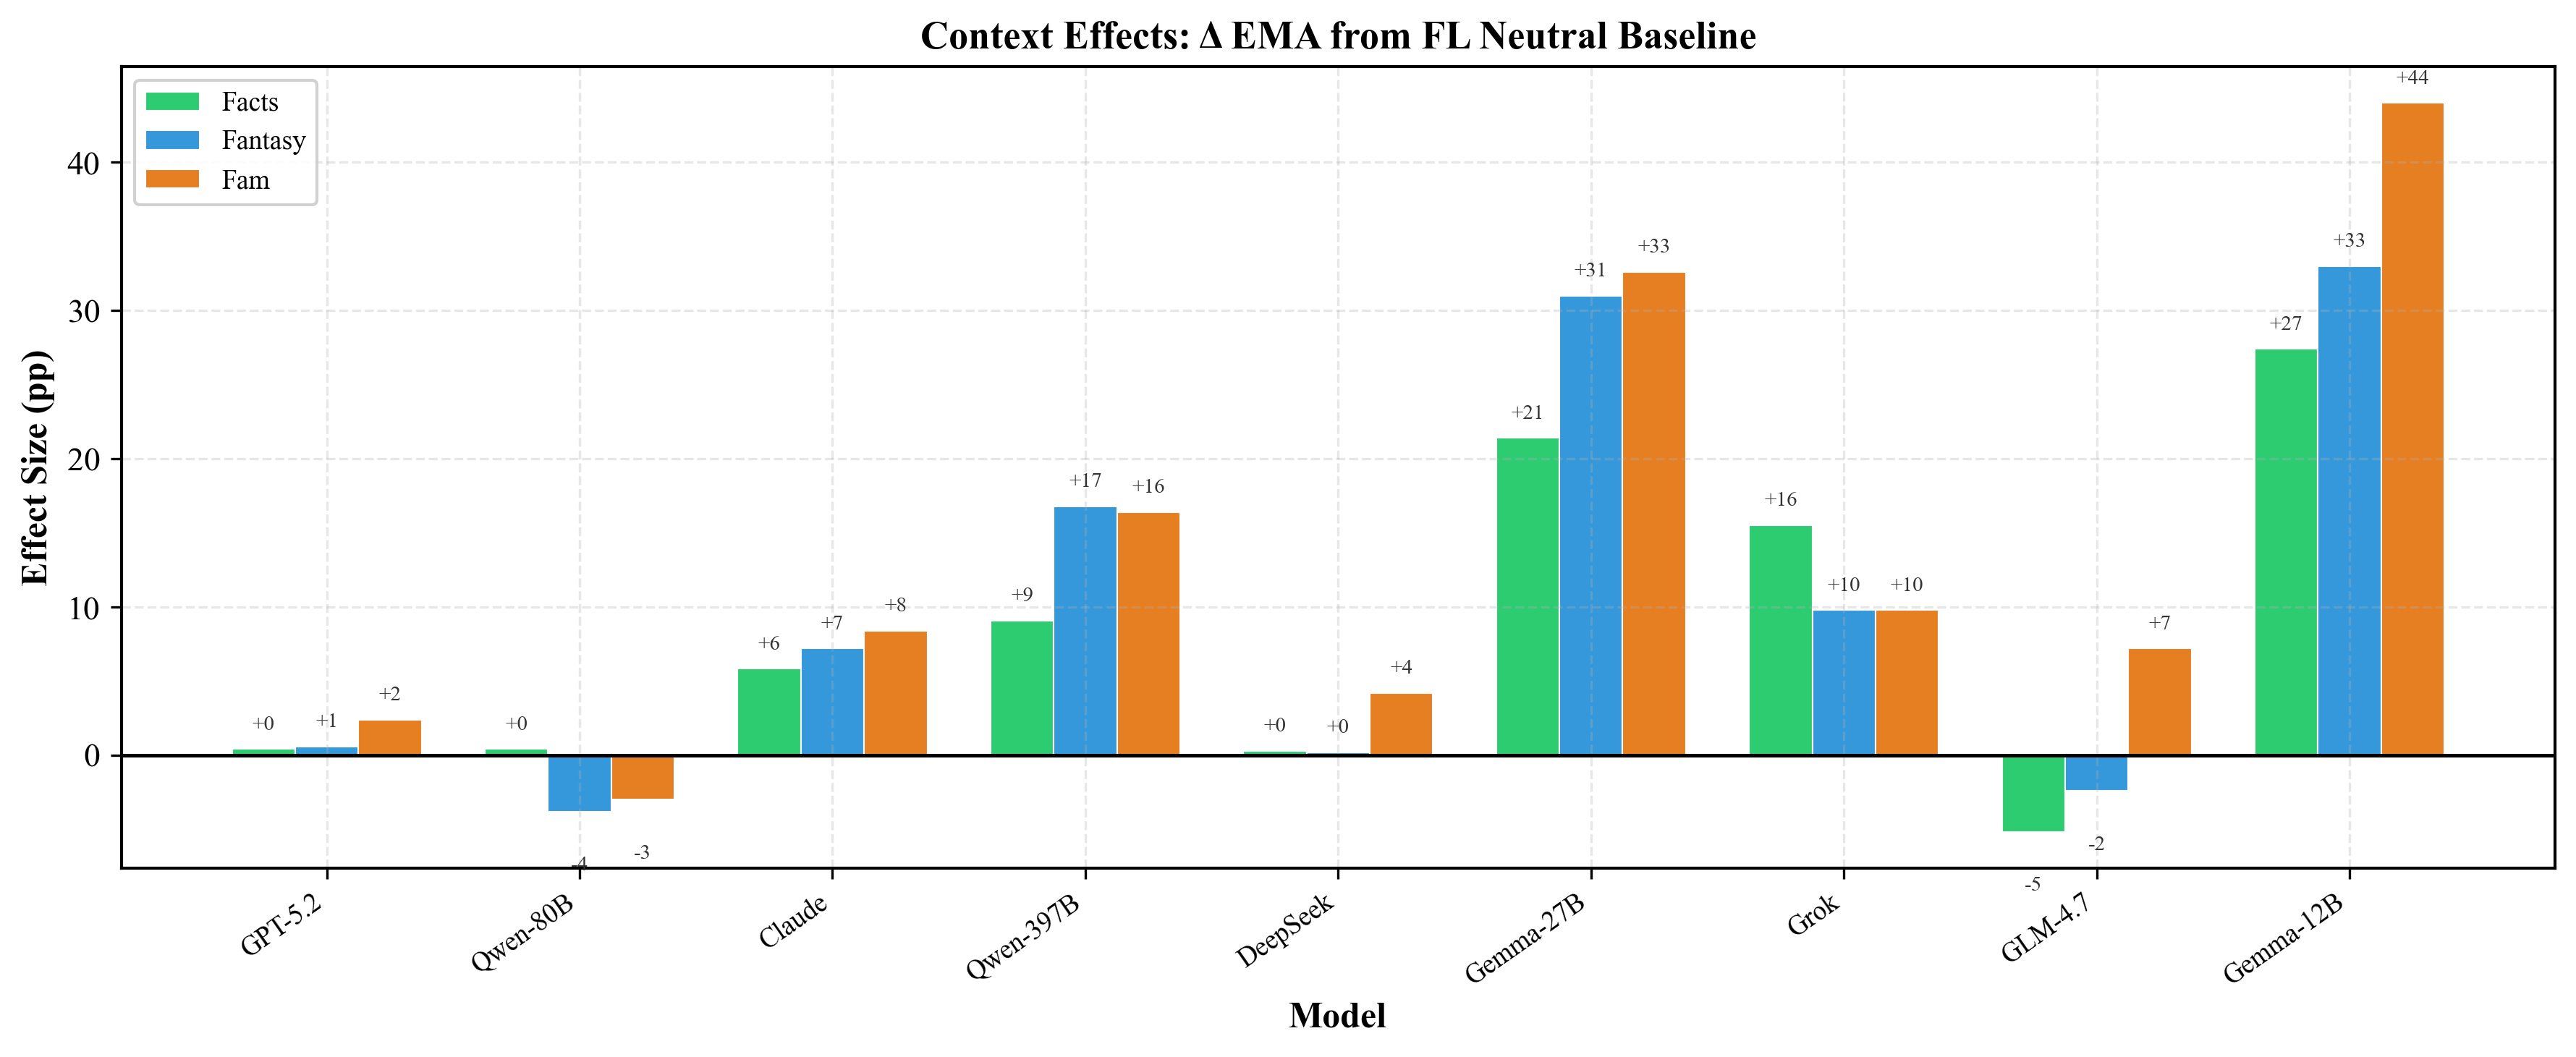
\includegraphics[width=0.85\textwidth]{../experiments_raw_results/wason-selection/figures/wason_context_effects.png}
\caption{Контент-эффект: изменение EMA при переходе от FL Neutral к Familiar Social Contracts (синий) и Unfamiliar Fantasy Social Contracts (оранжевый). Фасилитация наблюдается у всех моделей, причём Fantasy Social условия дают EMA, сопоставимый с Familiar Social, что подтверждает гипотезу деонтической структуры.}
\label{fig:context_effects}
\end{figure}

Исключением является \texttt{gemma-3-27b-it}, у которой EMA в условии Fantasy ($0{,}888$) лишь незначительно уступает Familiar ($0{,}904$), при этом EMA в нейтральном абстрактном условии ($0{,}578$) заметно ниже --- что указывает на особую чувствительность этой модели именно к деонтическому фреймингу, а не к знакомости содержания.

\textbf{Предубеждение подтверждения} подтверждено для всех моделей в нейтральном промпт-условии. В Formal Logic Neutral \texttt{gemma-3-12b-it} демонстрирует совокупный индекс bias (MBI + CBR) $= 0{,}536$ при EMA $= 0{,}106$ --- модель выбирает предубеждённый ответ в 5 раз чаще правильного, причём доминирующей ошибкой является Matching Bias ($0{,}516$). У \texttt{glm-4.7-flash} MBI $= 0{,}190$, CBR $= 0{,}040$ при EMA $= 0{,}614$; у \texttt{gemma-3-27b-it} MBI $= 0{,}296$ при EMA $= 0{,}578$. В контрасте, у моделей-лидеров MBI не превышает $0{,}020$ (кроме \texttt{claude-sonnet-4.6} с MBI $= 0{,}078$), а CBR равен нулю у пяти из девяти моделей. Важно, что контент-эффект снижает bias: переход к Familiar Social уменьшает MBI у \texttt{gemma-3-12b-it} с $0{,}516$ до $0{,}144$, а у \texttt{gemma-3-27b-it} --- с $0{,}296$ до $0{,}086$.

\begin{table}[h!]
\caption{MBI и CBR по пяти контентным условиям}
\label{tab:wst_bias}
\centering
\begin{tabular}{|l|cc|cc|cc|cc|cc|}
\hline
\multirow{2}{*}{\textbf{Модель}} & \multicolumn{2}{c|}{\textbf{FL Canon}} & \multicolumn{2}{c|}{\textbf{FL Neutral}} & \multicolumn{2}{c|}{\textbf{Conc. Facts}} & \multicolumn{2}{c|}{\textbf{Fam. Social}} & \multicolumn{2}{c|}{\textbf{Unf. Fantasy}} \\
\cline{2-11}
 & MBI & CBR & MBI & CBR & MBI & CBR & MBI & CBR & MBI & CBR \\
\hline
gemma-3-12b-it    & 0,493 & 0,020 & 0,516 & 0,020 & 0,285 & 0,018 & 0,144 & 0,000 & 0,236 & 0,004 \\
glm-4.7-flash     & 0,293 & 0,027 & 0,190 & 0,040 & 0,275 & 0,053 & 0,262 & 0,002 & 0,334 & 0,000 \\
gemma-3-27b-it    & 0,267 & 0,000 & 0,296 & 0,000 & 0,182 & 0,000 & 0,086 & 0,000 & 0,102 & 0,002 \\
grok-4.1-fast     & 0,153 & 0,000 & 0,170 & 0,000 & 0,067 & 0,000 & 0,054 & 0,000 & 0,082 & 0,000 \\
claude-sonnet-4.6 & 0,080 & 0,000 & 0,078 & 0,000 & 0,026 & 0,000 & 0,006 & 0,000 & 0,024 & 0,000 \\
deepseek-v3.2     & 0,013 & 0,000 & 0,020 & 0,000 & 0,014 & 0,000 & 0,028 & 0,002 & 0,028 & 0,000 \\
qwen3-next-80b    & 0,060 & 0,000 & 0,014 & 0,000 & 0,006 & 0,000 & 0,032 & 0,000 & 0,030 & 0,000 \\
qwen3.5-397b-a17b & 0,000 & 0,000 & 0,012 & 0,002 & 0,004 & 0,000 & 0,000 & 0,000 & 0,004 & 0,000 \\
gpt-5.2           & 0,000 & 0,000 & 0,000 & 0,004 & 0,004 & 0,000 & 0,002 & 0,000 & 0,010 & 0,000 \\
\hline
\end{tabular}
\end{table}

\textbf{Сравнение с человеческой производительностью.} Результаты LLM интерпретируются относительно эмпирических бейзлайнов людей (таблица~\ref{tab:human_wason}). Таблица~\ref{tab:human_llm_comparison} сопоставляет ключевые метрики.

\begin{table}[h!]
\caption{Сравнение производительности LLM с эмпирическими данными людей в задаче выбора Уэйсона}
\label{tab:human_llm_comparison}
\centering
\begin{tabular}{|l|c|c|c|}
\hline
\textbf{Метрика} & \textbf{Люди (абстрактная)} & \textbf{LLM топ-3} & \textbf{LLM слабые\textsuperscript{*}} \\
\hline
EMA (правильный ответ) & 4--19\% & 90--98\% & 10--61\% \\
Matching bias (P+Q) & 39--45\% & 0--2\% & 19--52\% \\
Confirmation (только P) & 33--36\% & 0\% & 0--4\% \\
Контент-эффект (доступ $\rightarrow$ соц.) & $+45$ п.п. & $+3$--$15$ п.п. & $+9$--$+44$ п.п. \\
\hline
\end{tabular}
\\[2pt]
\raggedright\footnotesize\textsuperscript{*}\texttt{gemma-3-12b-it}, \texttt{glm-4.7-flash}, \texttt{gemma-3-27b-it} --- три модели с наименьшей EMA в FL Neutral.
\end{table}

Даже слабейшая из протестированных моделей (\texttt{gemma-3-12b-it}, EMA~=~10{,}6\%) демонстрирует производительность на уровне нижней границы человеческого диапазона (4--19\%), а топовые модели превосходят людей на порядок. Однако паттерн ошибок у слабых LLM качественно родственен человеческому: доминирующей ошибкой является matching bias ($\{$P, Q$\}$), составляющий 51{,}6\% ответов \texttt{gemma-3-12b-it} --- это превышает верхнюю границу человеческого диапазона (45\%), хотя качественный паттерн доминирования matching bias совпадает.

Контент-эффект воспроизводит человеческий паттерн: и люди, и LLM улучшаются при переходе от абстрактных правил к деонтическим (социальным контрактам). У людей прирост составляет $\approx$+45 процентных пунктов (19\% $\rightarrow$ 64\%); у LLM медианный прирост от FL Neutral к Familiar Social составляет $+0{,}084$ ($+8{,}4$ п.п.), а у наиболее уязвимых моделей --- до $+0{,}440$ у \texttt{gemma-3-12b-it}. Масштаб эффекта у людей больше, что объясняется существенно более низким базисом в абстрактном условии. Направление эффекта --- одинаковое: деонтическая структура фасилитирует нормативное рассуждение у обоих типов агентов.

\begin{table}[h!]
\caption{Сравнение промпт-условий на датасете Formal Logic Neutral}
\label{tab:wst_prompts}
\centering
\begin{tabular}{|l|c|c|c|c|c|c|}
\hline
\multirow{2}{*}{\textbf{Модель}} & \multicolumn{3}{c|}{\textbf{Neutral prompt}} & \multicolumn{3}{c|}{\textbf{CoT prompt}} \\
\cline{2-7}
 & EMA & MBI & CBR & EMA & MBI & CBR \\
\hline
gpt-5.2            & 0,884 & 0,056 & 0,002 & 0,976 & 0,006 & 0,006 \\
claude-sonnet-4.6  & 0,790 & 0,172 & 0,002 & 0,970 & 0,000 & 0,000 \\
qwen3-next-80b     & 0,772 & 0,038 & 0,024 & 0,880 & 0,000 & 0,004 \\
qwen3.5-397b-a17b  & 0,764 & 0,032 & 0,000 & 0,974 & 0,000 & 0,004 \\
deepseek-v3.2      & 0,658 & 0,200 & 0,002 & 0,936 & 0,000 & 0,002 \\
grok-4.1-fast      & 0,424 & 0,450 & 0,000 & 0,664 & 0,032 & 0,252 \\
gemma-3-27b-it     & 0,406 & 0,386 & 0,006 & 0,368 & 0,436 & 0,120 \\
glm-4.7-flash      & 0,332 & 0,304 & 0,248 & 0,258 & 0,086 & 0,548 \\
gemma-3-12b-it     & 0,028 & 0,270 & 0,134 & 0,186 & 0,468 & 0,230 \\
\hline
\end{tabular}
\end{table}

\textbf{Эффект CoT-промпта} является одним из наиболее содержательных результатов. КоТ-промт оценивался на тех же 500 испытаниях (100 правил $\times$ 5 перестановок) в условии FL Neutral для открытых и проприетарных моделей. Полный CoT delta представлен на рисунке~\ref{fig:cot_delta}.

\begin{figure}[h!]
\centering
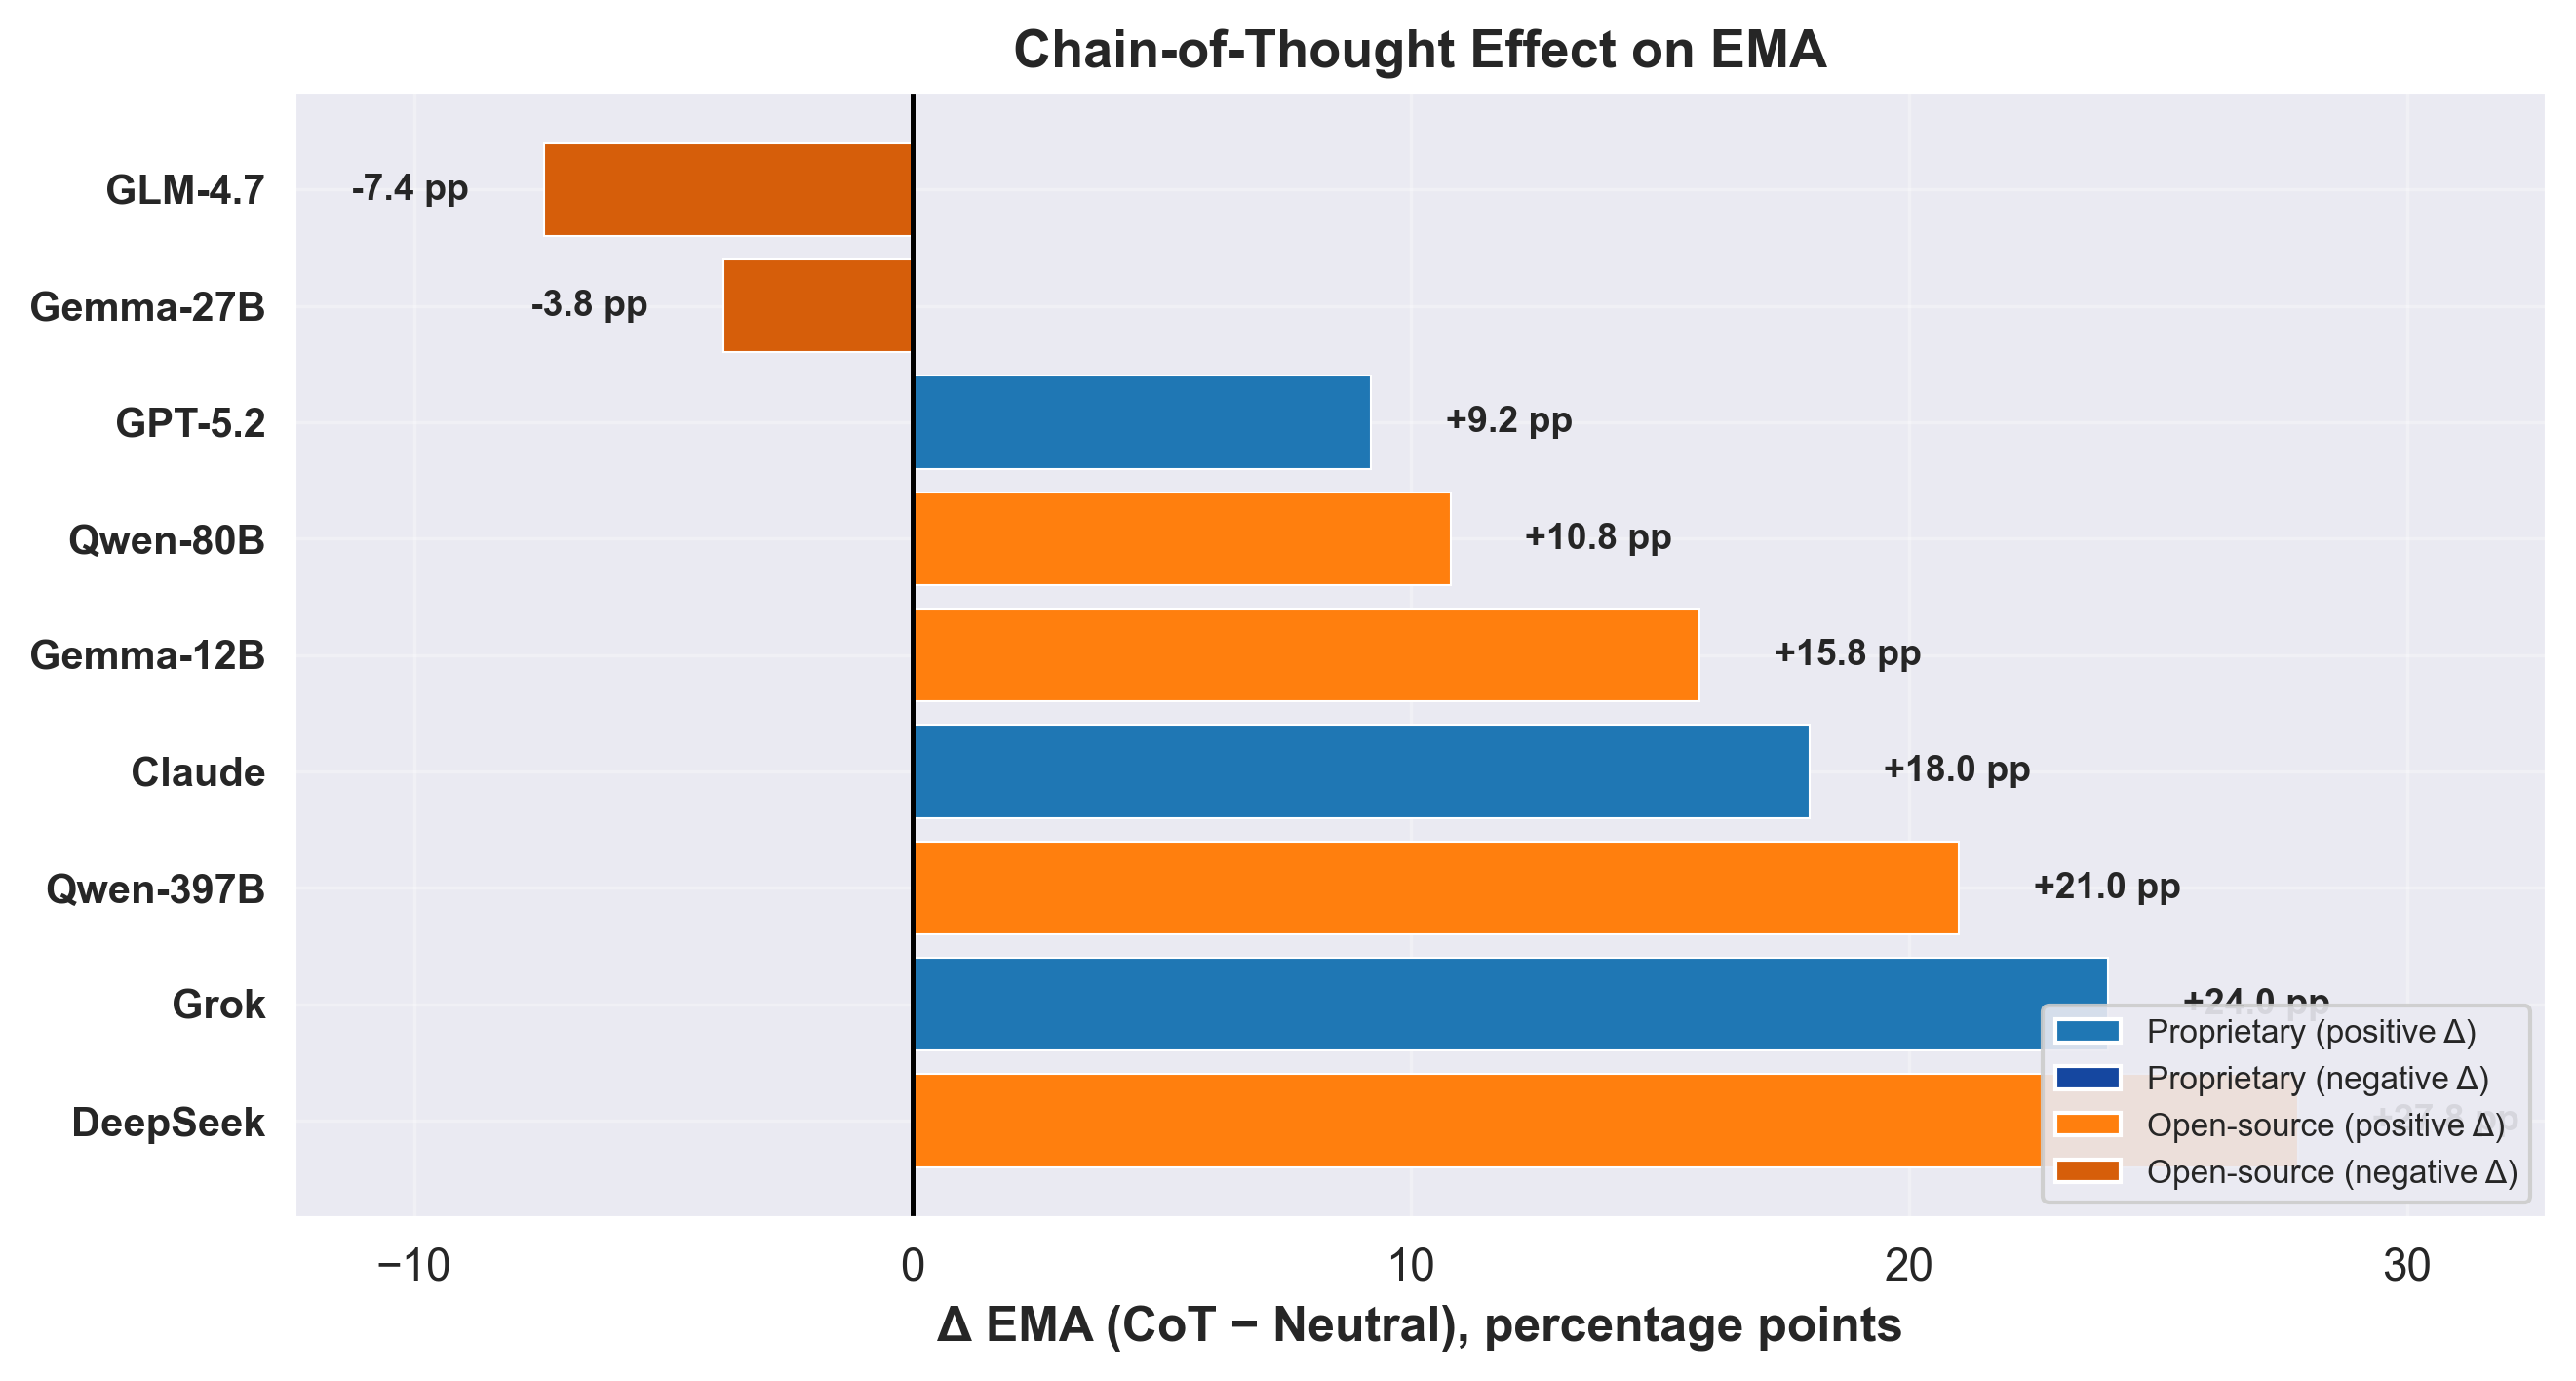
\includegraphics[width=0.85\textwidth]{../experiments_raw_results/wason-selection/output/thesis_graphs/wason_cot_delta.png}
\caption{CoT delta: изменение EMA при переходе от Neutral к CoT промпту. Для проприетарных моделей (синий) CoT даёт прирост у всех трёх моделей. Для открытых моделей (оранжевый) две модели демонстрируют отрицательный delta. Модели отсортированы по убыванию delta.}
\label{fig:cot_delta}
\end{figure}

Для проприетарных моделей CoT даёт положительный эффект у всех трёх: \texttt{grok-4.1-fast} (+0,240), \texttt{claude-sonnet-4.6} (+0,180), \texttt{gpt-5.2} (+0,092). При этом MBI и CBR у \texttt{claude} и \texttt{gpt-5.2} падают до нуля --- CoT не только повышает правильность, но и устраняет систематические ошибки.

Для открытых моделей картина дифференцирована. Четыре из шести показывают положительный delta: \texttt{deepseek-v3.2} (+0,278), \texttt{qwen3.5-397b-a17b} (+0,210), \texttt{gemma-3-12b-it} (+0,158), \texttt{qwen3-next-80b} (+0,108). Однако у \texttt{glm-4.7-flash} EMA снижается с 0,332 до 0,258 ($\Delta = -0{,}074$), а CBR вырастает с 0,248 до 0,548: явное рассуждение систематически приводит эту модель к выбору только карточки $\{$P$\}$ --- чистому confirmation bias. У \texttt{gemma-3-27b-it} CoT не меняет EMA содержательно (0,406 vs 0,368, $\Delta = -0{,}038$), однако перераспределяет ошибки: MBI растёт с 0,386 до 0,436, то есть явное рассуждение усиливает предубеждение соответствия. Это указывает на то, что CoT не является универсальным средством коррекции предубеждений и может давать обратный эффект у моделей с недостаточной базовой логической компетентностью~\cite{kojima2022large}.

\textbf{Стабильность ответов} в Formal Logic Neutral при нейтральном промпте варьирует от 0,110 у \texttt{gemma-3-12b-it} до 0,910 у \texttt{qwen3-next-80b}. Примечательно, что \texttt{qwen3-next-80b} демонстрирует наивысшую стабильность (0,910) при EMA 0,976 --- сочетание, нетипичное для других моделей. \texttt{gemma-3-27b-it} при EMA 0,578 имеет стабильность лишь 0,280 --- низкую относительно точности, что указывает на нестабильное угадывание, а не на систематическое рассуждение.

\begin{figure}[h!]
\centering
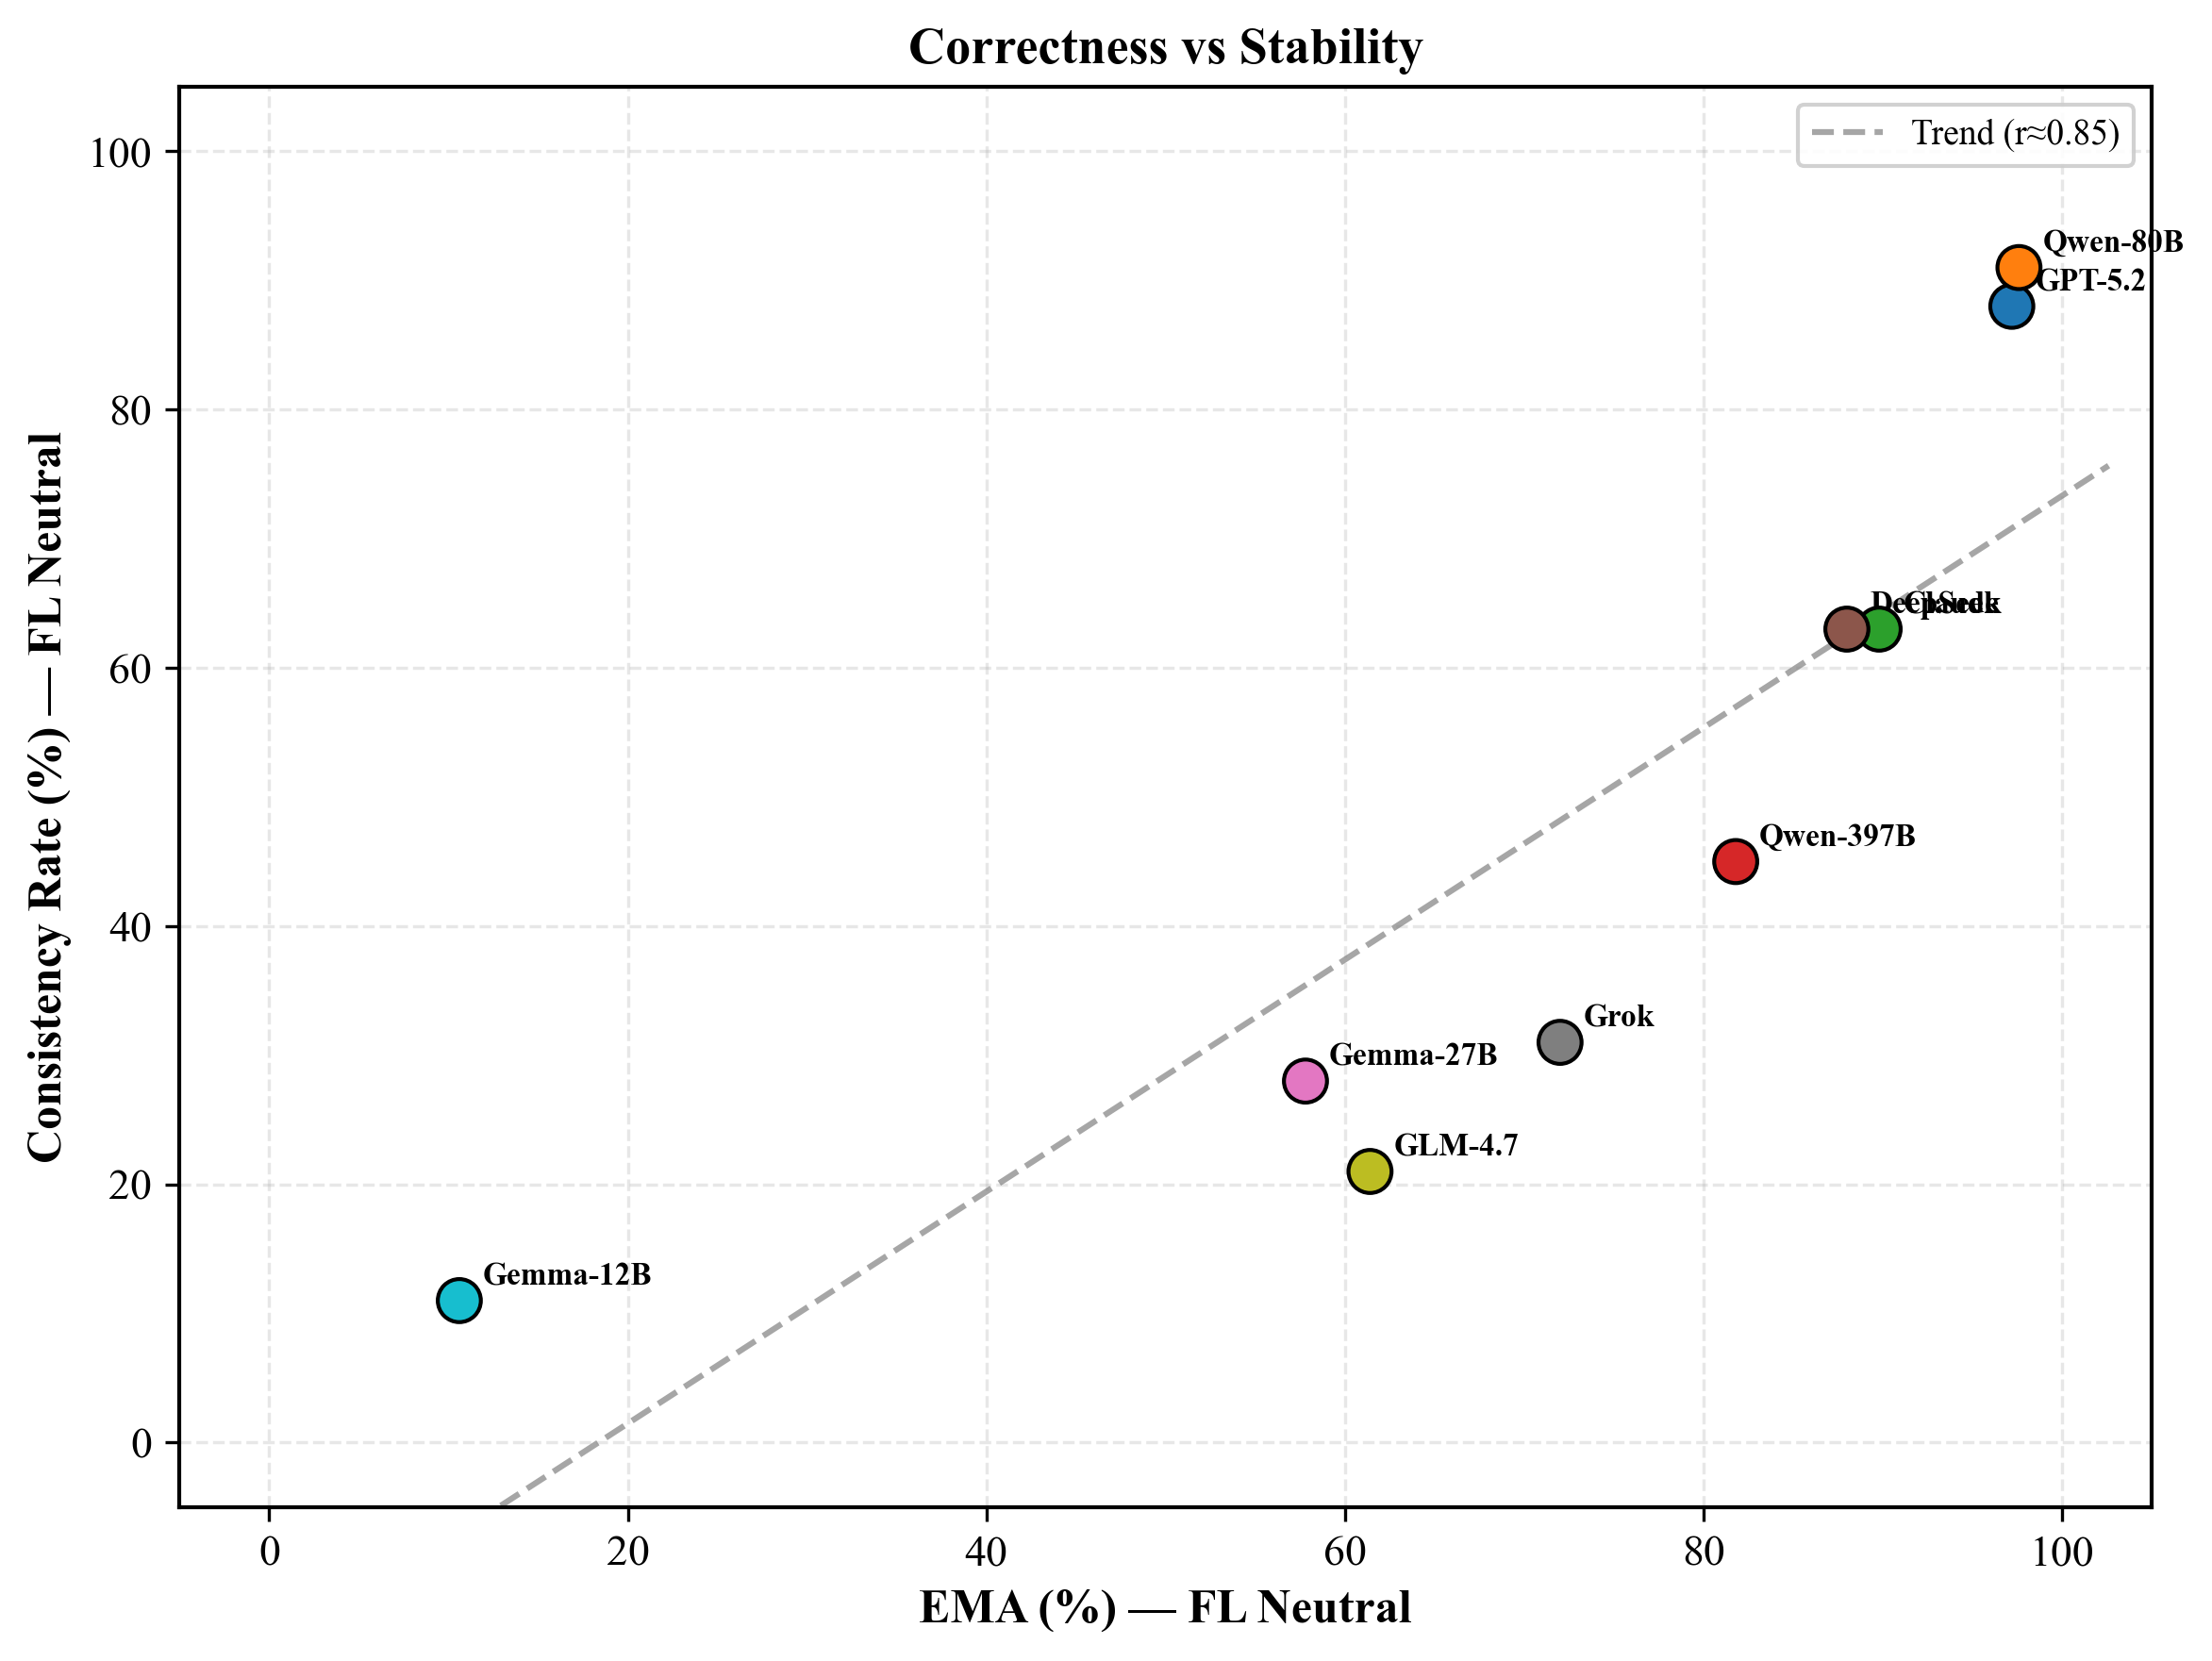
\includegraphics[width=0.85\textwidth]{../experiments_raw_results/wason-selection/figures/wason_ema_vs_consistency.png}
\caption{Связь EMA и Consistency Rate в FL Neutral. Идеальная модель находилась бы в правом верхнем углу (высокая точность + высокая стабильность). Топ-модели кластеризуются вблизи этого угла, в то время как слабые модели демонстрируют различные профили: низкая точность + низкая стабильность (\texttt{gemma-3-12b-it}), средняя точность + низкая стабильность (\texttt{gemma-3-27b-it}).}
\label{fig:ema_vs_consistency}
\end{figure}

\textbf{Внутрисемейный парадокс.} В семействе Gemma эффект из эксперимента 1 инвертируется: по EMA в Formal Logic Neutral \texttt{gemma-3-27b-it} ($0{,}578$) значительно превосходит \texttt{gemma-3-12b-it} ($0{,}106$). Таким образом, в вероятностной задаче 27b была более уязвима, чем 12b, а в логической задаче --- менее уязвима. Это указывает на то, что уязвимость к разным типам когнитивных предубеждений не определяется единым фактором и может иметь различную направленность в зависимости от типа рассуждения.

\subsection{Качественный анализ категорий ошибок}

Помимо агрегированных метрик, классификация ответов на шесть содержательных категорий позволяет детально описать паттерны ошибочного рассуждения. Ниже приведены категории, их частоты в FL Neutral (наиболее «чистом» условии) и типичные примеры.

\textbf{1. CORRECT} ($\{$P, $\lnot$Q$\}$). Нормативно правильный ответ. В FL Neutral варьирует от 10,6\% (\texttt{gemma-3-12b-it}) до 97,6\% (\texttt{qwen3-next-80b}).

\textbf{2. MATCHING BIAS} ($\{$P, Q$\}$). Выбор обеих карточек, явно упомянутых в правиле. Каноническая ошибка, описанная ещё у Evans~\cite{evans1998matching}. Доминирующая ошибка слабых моделей: \texttt{gemma-3-12b-it} допускает её в 51,6\% испытаний.

\begin{quote}
\textit{Правило:} «If there is an A on one side, then there is a 3 on the other side.»\\
\textit{Ответ gemma-3-12b-it:} \texttt{['A', '3']} — выбрала именно те карточки, что названы в правиле (P + Q).
\end{quote}

\textbf{3. CONFIRMATION BIAS} ($\{$P$\}$). Выбор только подтверждающей карточки, без проверки $\lnot$Q. Относительно редкая категория (0--4\% у большинства моделей), но существенная у \texttt{gemma-3-12b-it} (2,0\%) и \texttt{glm-4.7-flash} (4,0\%).

\begin{quote}
\textit{Правило:} «If there is a U on the card, then there is an 8 on the back.»\\
\textit{Ответ gemma-3-12b-it:} \texttt{['U']} --- единственная P, игнорирует необходимость проверки $\lnot$Q.
\end{quote}

\textbf{4. LOGIC ERROR} (другие неправильные комбинации). Включает выбор $\{$not\_P, not\_Q$\}$, $\{$not\_P, Q$\}$, одиночных $\{$Q$\}$ или $\{$not\_Q$\}$ и другие неклассифицируемые ответы. Вторая по частоте ошибка после matching bias.

\begin{quote}
\textit{Правило:} «If the number is 6, then the letter is S.»\\
\textit{Ответ gemma-3-12b-it:} \texttt{['9', 'P']} — выбрала not\_P + not\_Q, что является полной инверсией логики.
\end{quote}

\textbf{5. OVER-SELECTION} (более 2 карточек, но не все 4). Редкая категория (0,4--2,2\%), встречается преимущественно у слабых моделей при деонтическом контенте.

\begin{quote}
\textit{Правило:} «If the element is Gold, then it does not Rust.»\\
\textit{Ответ glm-4.7-flash:} \texttt{['Gold', 'Does not rust', 'Iron']} --- 3 карточки, попытка «перестраховаться».
\end{quote}

\textbf{6. ALL CARDS} (все 4 карточки). Крайняя форма неопределённости: модель выбирает все доступные карточки. Встречается в 0,2--1,1\% испытаний.

\begin{quote}
\textit{Правило:} «If the animal is a Camel, then it has a Hump.»\\
\textit{Ответ gemma-3-12b-it:} \texttt{['Camel', 'Hump', 'Horse', 'No hump']} --- все 4 карточки.
\end{quote}

Совокупное распределение категорий в FL Neutral отражает иерархию компетентности: у \texttt{gemma-3-12b-it} 51,6\% Matching Bias + 11,1\% Logic Error + 2,0\% Confirmation Bias = 64,7\% ошибок трёх главных типов, в то время как у \texttt{gpt-5.2} 0,0\% + 2,4\% + 0,4\% = 2,8\%.

\subsection{Выводы по эксперименту 2}

Эксперимент 2 установил:

\begin{enumerate}
  \item \textbf{Предубеждение подтверждения} в дедуктивном рассуждении у всех девяти моделей в нейтральном условии. Совокупный индекс bias (MBI + CBR) варьирует от 0,4\% у \texttt{gpt-5.2} до 53,6\% у \texttt{gemma-3-12b-it}, причём доминирующей ошибкой является matching bias, а не confirmation bias в строгом смысле.

  \item \textbf{Устойчивый контент-эффект} --- социальные контракты решаются значимо лучше абстрактных правил у 8 из 9 моделей (медианный прирост EMA $+0{,}084$). Переход к Familiar Social одновременно снижает MBI: у \texttt{gemma-3-12b-it} с $0{,}516$ до $0{,}144$.

  \item \textbf{Поддержка гипотезы прагматических схем} Ченга-Холиоака через условие фантастических социальных контрактов, которое даёт EMA, сопоставимое со знакомыми контрактами (медианный прирост от FL Neutral $+0{,}072$). Деонтическая структура обязательства фасилитирует логический вывод независимо от знакомости содержания.

  \item \textbf{Дифференцированный эффект CoT} --- проприетарные модели все улучшаются (median $\Delta = +0{,}180$), тогда как 2 из 6 открытых моделей показывают отрицательный delta: \texttt{glm-4.7-flash} ($-0{,}074$) и \texttt{gemma-3-27b-it} ($-0{,}038$). CoT не является универсальной коррекцией предубеждений.

  \item \textbf{Инверсия внутрисемейного парадокса Gemma} по сравнению с экспериментом 1: 27b превосходит 12b в логической задаче, но была более уязвима в вероятностной, что свидетельствует о мультидимензиональности когнитивных предубеждений.

  \item \textbf{Шесть качественных категорий ошибок}, из которых matching bias доминирует у слабых моделей (до 51,6\%), в то время как confirmation bias в строгом смысле (выбор только P) составляет 0--4\% у большинства моделей.

  \item \textbf{Сравнение с человеческой производительностью.} Топовые модели превосходят людей на порядок по EMA (90--98\% vs 4--19\%), однако слабые модели воспроизводят качественно аналогичный паттерн ошибок: доминирование matching bias, низкий уровень строгого confirmation bias, а также положительный контент-эффект при деонтическом framing. Направление контент-эффекта совпадает у людей и LLM, но масштаб различается из-за разного базиса в абстрактном условии.
\end{enumerate}

